\documentclass{article}
\usepackage[landscape]{geometry}
\usepackage{url}
\usepackage{multicol}
\usepackage{amsmath}
\usepackage{esint}
\usepackage{bigints}
\usepackage{amsfonts}
\usepackage{xcolor}
\usepackage{tikz}
\usetikzlibrary{calc}
\usetikzlibrary{decorations.pathmorphing}
\usepackage{amssymb}
\usepackage{bm}
\usepackage{physics}
\usepackage[export]{adjustbox}

\DeclareMathOperator{\Jinc}{Jinc}
\DeclareMathOperator{\sinc}{sinc}
\DeclareMathOperator{\rect}{rect}
\DeclareMathOperator{\tri}{tri}

\usepackage{colortbl}
\usepackage{xcolor}
\usepackage{mathtools}
\usepackage{xhfill}
\makeatletter

\newcommand*\bigcdot{\mathpalette\bigcdot@{.5}}
\newcommand*\bigcdot@[2]{\mathbin{\vcenter{\hbox{\scalebox{#2}{$\m@th#1\bullet$}}}}}
\makeatother

\usepackage{polyglossia}
\setdefaultlanguage{hebrew}
\setotherlanguage{english}
\setotherlanguage{french}
% Fonts
\setmainfont{David CLM}
\setsansfont{Liberation Sans}
\setmonofont{Liberation Mono}
\newfontfamily\hebrewfont{David CLM}[Script=Hebrew]
\newfontfamily\hebrewfontsf{Liberation Serif}[Script=Hebrew]
\newfontfamily\hebrewfonttt{Liberation Mono}[Script=Hebrew]
\newfontfamily\frenchfont{Cardo}
\newfontfamily\frenchfontsf{Cardo}
\newfontfamily\frenchfonttt{Cardo}
% to fix itemize lists:
% https://tex.stackexchange.com/a/53453/125609
\usepackage{enumitem}
\setlist[itemize,1]{label={\fontfamily{cmr}\fontencoding{T1}\selectfont\textbullet}}

% For Pariente
\usepackage{tikzlings-cats}

%cambios de unidades (pt, mm, cm,ex,em,bp,dd,pc,sp) https://tex.stackexchange.com/questions/8260/what-are-the-various-units-ex-em-in-pt-bp-dd-pc-expressed-in-mm
\advance\topmargin-.8in
\advance\textheight3in
\advance\textwidth3in
\advance\oddsidemargin-1.5in
\advance\evensidemargin-1.5in
\parindent0pt
\parskip2pt
\newcommand{\hr}{\centerline{\rule{3.5in}{1pt}}}
\newcommand{\nc}[2][]{
\tikz \draw [draw=black, ultra thick, #1]
    ($(current page.center)-(0.5\linewidth,0)$) -- 
    ($(current page.center)+(0.5\linewidth,0)$)
    node [midway, fill=white] {#2};
}% tomado de https://tex.stackexchange.com/questions/179425/a-new-command-of-the-form-tex

\title{אופטיקה עם יואב שגיא - נוסחאון}

\begin{document}

%\begin{center}
% Not using \maketitle because it uses too much space on page
%אופטיקה עם יואב שגיא - נוסחאון
%\end{center}
\begin{multicols*}{3}

\tikzstyle{mybox} = [draw=black, fill=white, very thick,
    rectangle, rounded corners, inner sep=10pt, inner ysep=10pt]
\tikzstyle{fancytitle} =[fill=black, text=white, font=\bfseries]

%--------------------------
\begin{tikzpicture}
\node [mybox] (box){
\begin{minipage}{0.3\textwidth}
\begin{hebrew}\textbf{
באופן כללי:
}\end{hebrew}
$$
\begin{array}{ll}
    \div{\vb{E}} = \rho/\epsilon_0 & \displaystyle \curl{\vb{E}} = -\pdv{\vb{B}}{t} \\
    \div{\vb{B}} = 0               & \displaystyle \curl{\vb{B}} = \mu_0 \vb{J} + \mu_0 \epsilon_0 \pdv{\vb{E}}{t}
\end{array}
$$
\begin{hebrew}\textbf{
בחומר:
}\end{hebrew}
$$
\begin{array}{ll}
    \displaystyle \div{\vb{D}} = \rho_{free}          & \displaystyle \curl{\vb{E}} = -\pdv{\vb{B}}{t} \\
    \displaystyle \div{\vb{B}} = 0                    & \displaystyle \curl{\vb{H}} = \vb{J_{free}} + \pdv{\vb{D}}{t} \\
    \displaystyle \vb{D} = \epsilon_0 \vb{E} + \vb{P} & \displaystyle \vb{H} = \frac{1}{\mu_0}\vb{B} - \vb{M}
\end{array}
$$
\begin{hebrew}\textbf{
בחומר לינארי:
}\end{hebrew}
$$
\begin{array}{ll}
    \displaystyle \vb{P} = \epsilon_0 \chi_e \vb{E}                          &
    \displaystyle \vb{M} = \chi_m \vb{H} \\
    \displaystyle \vb{D} = \epsilon_0 ( 1 + \chi_e) \vb{E} = \epsilon \vb{E} &
    \displaystyle \vb{H} = \frac{1}{\mu_0}(1 + \chi_m) \vb{B} = \frac{1}{\mu} \vb{B}
\end{array}
$$
\begin{hebrew}\textbf{
משוואת הגלים בחומר:
}\end{hebrew}

$$
\begin{array}{ll}
    \displaystyle \laplacian{\vb{E}} = \mu \epsilon \pdv[2]{\vb{E}}{t} & \displaystyle \laplacian{\vb{H}} = \mu \epsilon \pdv[2]{\vb{H}}{t}
\end{array}
$$

\begin{hebrew}
\underline{
פתרון:
}
$$\vb{E} = \vb{E_0} \exp(\pm i (\vb{k} \dotproduct \vb{r} - \omega t))$$
$$\vb{H} = \frac{1}{\eta} \cdot \vu{k}\cross\vb{E_0} \exp(\pm i (\vb{k} \dotproduct \vb{r} - \omega t))$$
$$\expval{\vb{S}} = \frac{\real\mathrm{e}\{\vu{k}\}}{2\eta} \exp(-2 \imaginary\mathrm{m}\{\vb{k}\}\dotproduct \vb{r}) \abs{\vb{E_0}}^2$$

\vspace{-1em}

\underline{
הנחות:
}
\begin{itemize}
    \item חומר לינארי עם
$\chi_e$
ו-
$\chi_m$
לא תלויים בזמן.
    \item $\rho_{free} = 0, \vb{J}_{free} = 0$
\end{itemize}
\underline{
הגדרות:
}
\end{hebrew}
\begin{english}
$$
\begin{array}{rclrcll}
    \epsilon_m & = & 1 + \chi_m & c_0 & = & 1/\sqrt{\epsilon_0 \mu_0} & n = c_0/c \\
    \epsilon_r & = & 1 + \chi_e & c & = & 1/\sqrt{\epsilon \mu}       & n = \sqrt{\epsilon_r \mu_r} \\
\end{array}
$$
$$
\begin{array}{rcl}
\eta = \sqrt{\mu/\epsilon} &=& \text{Wave Impedance} \\
\omega = c \abs{\vb{k}} &=& \text{Dispersion Relation} \\
\lambda = 2\pi / \abs{\vb{k}} &=& \text{Wave Length} \\
\vb{S}_{microscopic} = \frac{1}{\mu_0}\vb{E}\cross\vb{B} &=& \text{Poynting vector} \\
\expval{\vb{S}} &=& \frac{1}{2}\real\mathrm{e}\{\vb{E}\cross\vb{H}^*\}
\end{array}
$$
$$ [\vb{S}] = \frac{\text{Power (Watt)}}{\text{Area}(m^2)}, [\eta] = \Omega , \omega = 2\pi f, [f] = Hz$$
\end{english}

\vspace{-1em}

\end{minipage}
};
\node[fancytitle, left=10pt] at (box.north east) {\foreignlanguage{hebrew}{
משוואות מקסוול
(\textbf{SI})
}};
\end{tikzpicture}

%---------------------------
\begin{tikzpicture}
\node [mybox] (box){
    \begin{minipage}{0.3\textwidth}\begin{hebrew}\foreignlanguage{hebrew}{
    \nc{\foreignlanguage{hebrew}{
    מודל לורנץ - אוסילטור הרמוני
    }}
    האלקטרון קשור לאטום כמו מסה עם קפיץ:
    $$\vb{F} = q \vb{E} = m (\ddot{\vb{x}}+\gamma \dot{\vb{x}}+\omega_0^2 \vb{x})$$
    $\omega_0$ -
    תדר של אנרגית מעבר בין רמות. הפולאריזביליות:
    $$\vb{P} = n \vb{p} = N q \vb{x}(\omega) = N \epsilon_0 \alpha(\omega) \vb{E}(\omega) = \epsilon_0 \chi(\omega) \vb{E}(\omega)$$
    מציבים פתרון פאזורי 
    $\vb{E}(\omega) = \vb{E}_0 \exp(i \omega t)$
    ומקבלים:
    $$\chi(\omega) = \frac{\omega_p^2}{\omega_0^2 - \omega^2 + i \gamma \omega}$$
    כאשר:
    $\omega_p^2 = \frac{N q^2}{m \epsilon_0}$ -
    תדירות הפלאזמה,
    $N$ -
    צפיפות האלקטרונים בחומר. מקובל לכתוב גם:
    $$\chi(\omega) \equiv \chi'(\omega) - i \chi''(\omega)$$
    $$\begin{array}{rcl}
    	\chi'(\omega) &=&
	\frac{\omega_p^2\left(\omega_0^2 - \omega^2\right)}{\left(\omega_0^2 - \omega^2\right)^2 + (\gamma \omega)^2} \\
    	\chi''(\omega) &=&
	\frac{\omega_p^2\left(i \gamma \omega \right)}{\left(\omega_0^2 - \omega^2\right)^2 + (\gamma \omega)^2}
    \end{array}$$
    \nc{Clausius-Mosotti}
    מתבסס על מודל לורנץ, אך לוקח בחשבון אינטראקציה בין הדיפולים. משתמשים ב-
    $\alpha(\omega) = \chi(\omega)/N$
    ממודל לורנץ ובביטוי מעט שונה ל-$\vb{P}$:
    $$
    \vb{P} =
    \frac{N \alpha(\omega)}{1 - \frac{N \alpha(\omega)}{3}}
    \cdot \epsilon_0 \vb{E}(\omega)$$
    $$
    n(\omega) = \sqrt{\epsilon_r \mu_r}\approx \sqrt{\epsilon_r} = \sqrt{
    1 + \frac{N \alpha(\omega)}{1 - \frac{N \alpha(\omega)}{3}}
    }
    $$
    \nc{\foreignlanguage{hebrew}{
    הפרשי פאזה
    }}
    \vspace{-1em}
    $$\begin{array}{lcr}
    	\angle \frac{P}{E} = \arctan(-\frac{\chi''}{\chi'}) & &
	\angle \frac{B}{E} \overset{\chi'' \ll \chi'}{\approx}
	-\frac{1}{2} \arctan(\frac{\chi''}{1+\chi'})
    \end{array}$$
    \nc{\foreignlanguage{hebrew}{
    מתכות: לורנץ + דרודה
    }}
    \vspace{-1em}
    $$\begin{array}{lcccr}
    	\omega_0 \overset{Metals}{\rightarrow} 0 & & \dot{\vb{x}} \overset{Drude}{=} q \vb{E} \sigma/N & & \chi(\omega) = \frac{\omega_p^2}{i \omega \gamma - \omega^2}
    \end{array}$$
    }\end{hebrew}
    \end{minipage}
};
\node[fancytitle, left=10pt] at (box.north east) {\foreignlanguage{hebrew}{
מקדם שבירה - מודלים
}};
\end{tikzpicture}

%---------------------------
\begin{tikzpicture}
\node [mybox] (box){
    \begin{minipage}{0.3\textwidth}\foreignlanguage{hebrew}{
$$\laplacian{\vb{E}} = \mu_0 \sigma \pdv{\vb{E}}{t} + \mu_0 \epsilon \pdv[2]{\vb{E}}{t}$$
\underline{
הנחות:
}
\begin{itemize}
    \item חומר לינארי עם
$\chi_e$
ו-
$\chi_m = 0 \Rightarrow \mu = \mu_0$
    \item $\rho_{free} = 0$, $\vb{J}_{free} \overset{Ohm}{=} \sigma \vb{E} \ne 0$
\end{itemize}
\underline{
פתרון:
}
$\vb{E}, \vb{H}, \expval{\vb{S}}$ - כמו בחומר דיאלקטרי, אבל:
$$k = \omega \sqrt{\mu_0 \epsilon} \sqrt{1 - i \frac{\sigma}{\epsilon \omega}} \Rightarrow
\eta =\frac{\omega \mu_0}{k} = \sqrt{\frac{\mu_0}{\epsilon}}\frac{1}{\sqrt{1 - i \frac{\sigma}{\epsilon \omega}}}$$
נגדיר
$k = \frac{2\pi}{\lambda_m} - \frac{i}{\delta}$
כאשר
$\delta$ -
עומק החדירה,
$\lambda_m$ -
אורך הגל במתכת. עבור אור נראה:
$\omega \ll \omega_p^2/\gamma$
ולכן:

$$\lambda_m \approx 2\pi \sqrt{\frac{2}{\omega \mu_0 \sigma}} \approx 2 \pi \delta $$

}\end{minipage}
};
\node[fancytitle, left=10pt] at (box.north east) {\foreignlanguage{hebrew}{
משוואות מקסוול במתכות
}};
\end{tikzpicture}

%---------------------------
\begin{tikzpicture}
\node [mybox] (box){
\begin{minipage}{0.3\textwidth}\foreignlanguage{hebrew}{
\nc{\foreignlanguage{hebrew}{
משוואת האליפסה
}}
נניח גל המתקדם בכיוון
$\hat{z}$:

\vspace*{-1.5em}
$$\begin{array}{lcr}
\vb{E} =
\real\mathrm{e}\bigg\{E_0 \left (\alpha \hat{x} + \beta \hat{y}\right)e^{i (\omega t -k z)} \bigg\}
& &
\abs{\alpha}^2 + \abs{\beta}^2 = 1
\end{array}$$

עם
$\delta$
פאזה יחסית בין
$\alpha$
ל-
$\beta$,
נגדיר:

$$\begin{array}{lr}
    E_x \equiv E_0 \abs{\alpha} \cos(\omega t - k z) &
    A \equiv \frac{E_x}{E_0 \abs{\alpha}} \\
    E_y \equiv E_0 \abs{\beta} \cos(\omega t - k z + \delta) &
    B \equiv \frac{E_y}{E_0 \abs{\beta}}
\end{array}$$

נקבל:

$$A^2 - 2 A B \cos(\delta) + B^2 = \sin^2(\delta)$$

$$\begin{array}{lr}
    \delta = 0, \pm \pi \Rightarrow \text{\textenglish{Linear}} &
    \delta = \pm \pi/2 \Rightarrow \text{\textenglish{Circular}}
\end{array}$$

נוכל לבחור לייצג את
$\alpha \hat{x} + \beta \hat{y}$
באמצעות
$\hat{\epsilon}_1, \hat{\epsilon}_2$
המקיימים
$\hat{\epsilon}_1\dotproduct \hat{\epsilon}_2^* = 0$
למשל:

$$\begin{array}{lr}
    \begin{cases}
    \hat{\epsilon}_1 = \hat{x} \\
    \hat{\epsilon}_2 = \hat{y}
    \end{cases}
    &
    \begin{cases}
    \displaystyle \hat{\epsilon}_R = \frac{\hat{x} - i \hat{y}}{\sqrt{2}} \\
    \displaystyle \hat{\epsilon}_L =  \frac{\hat{x} + i \hat{y}}{\sqrt{2}}
    \end{cases}
\end{array}$$

}\end{minipage}
};
\node[fancytitle, left=10pt] at (box.north east) {\foreignlanguage{hebrew}{
קיטובים
}};
\end{tikzpicture}

%---------------------------
\begin{tikzpicture}
\node [mybox] (box){
\begin{minipage}{0.3\textwidth}\foreignlanguage{hebrew}{
\nc{\foreignlanguage{hebrew}{
וקטור \textenglish{Jones}
}}
\vspace*{-1.5em}
נבחר בסיס של
$\hat{\epsilon}_1, \hat{\epsilon}_2$
וניקח
$a,b\in \mathbb{C}$
כך ש:

$$\begin{array}{lcr}
\vb{E} =
\real\mathrm{e}\bigg\{E_0 \left (a \hat{\epsilon_1} + b \hat{\epsilon_2}\right)e^{i (\omega t -k z)} \bigg\}
& \Rightarrow & \vb{J} = \mqty(a \\ b)
\end{array}$$

\nc{\foreignlanguage{hebrew}{
כדור
\foreignlanguage{french}{Poincaré}
}}
\vspace*{-1.5em}

עבור
$\hat{\epsilon_1} = \hat{x}, \hat{\epsilon_2} = \hat{y}$
ו-
$\vb{J}$
נגדיר וקטור ממשי:

$$\vb{S} = \big (
    \abs{a}^2 - \abs{b}^2,
    2\real\mathrm{e}\{a^* b \},
    2\imaginary\mathrm{m}\{a^* b \}
\big ) $$

}\end{minipage}
};
\node[fancytitle, left=10pt] at (box.north east) {\foreignlanguage{hebrew}{
קיטובים
}};
\end{tikzpicture}

%---------------------------
\begin{tikzpicture}
\node [mybox] (box){
\begin{minipage}{0.3\textwidth}
    \begin{center}
    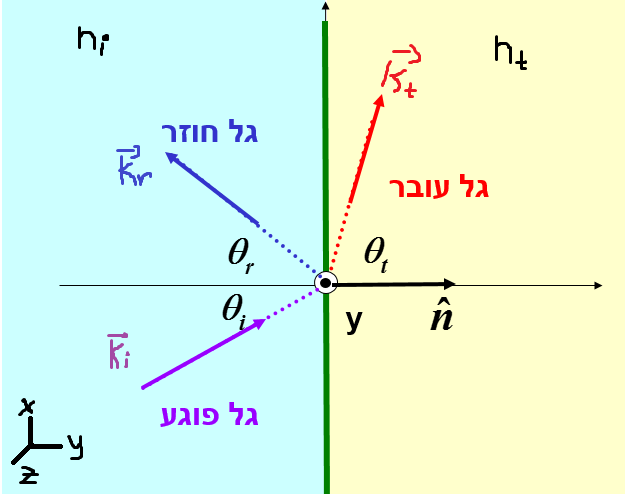
\includegraphics[width=0.85\textwidth]{./fresnel-setup.png}
    \end{center}
    \vspace*{-3em}
    \foreignlanguage{hebrew}{
    \begin{itemize}
        \item $\vb{E}$
    	\textbf{מוכל}
    	במישור הפגיעה
    	$\Leftarrow$
    	קיטוב
    	\textbf{מקביל}
    	= קיטוב
    	"\textbf{$P$}"
	    \item $\vb{E}$
	    \textbf{ניצב}
	    למישור הפגיעה
	    $\Leftarrow$
	    קיטוב
	    \textbf{ניצב} 
	    = קיטוב
	    "\textbf{$S$}"
    \end{itemize}
    משוואות רציפות והגדרות:
    $$\begin{array}{lcl}
    	\vu{n} \cross \left(\vb{E}_1 - \vb{E_2}\right) = 0 & & \vu{n} \dotproduct \left( \vb{D}_2 - \vb{D}_1 \right ) = 0 \\
    	\vu{n} \cross \left(\vb{H}_1 - \vb{H}_2 \right) = 0 & & \vu{n} \dotproduct \left( \vb{B}_2 - \vb{B}_1 \right ) = 0
    \end{array}$$
    $$\begin{array}{lclcl}
    	\displaystyle r_s = \frac{E_{r,s}}{E_{i,s}} & & \displaystyle \vb{E}_1 = \vb{E}_i + \vb{E}_r                   & & \displaystyle \vb{E}_2 = \vb{E}_t \\
    	\displaystyle t_s = \frac{E_{t,s}}{E_{i,s}} & & \displaystyle \vb{D}_1 = \epsilon_i (\vb{E}_i + \vb{E}_r)      & & \displaystyle \vb{D}_2 = \epsilon_t \vb{E}_t \\
    	\displaystyle r_p = \frac{E_{r,p}}{E_{i,p}} & & \displaystyle \vb{H}_1 = \frac{1}{\mu_i} (\vb{B}_i + \vb{B}_r) & & \displaystyle \vb{H}_2 = \frac{1}{\mu_t} \vb{B}_t \\
    	\displaystyle t_p = \frac{E_{t,p}}{E_{i,p}} & & \displaystyle \vb{B}_1 = \vb{E}_i + \vb{E}_r                   & & \displaystyle \vb{E}_2 = \vb{E}_t
    \end{array}$$
    }
\end{minipage}
};
\node[fancytitle, left=10pt] at (box.north east) {\foreignlanguage{hebrew}{
מעבר בין תווכים ומשוואות
\textenglish{Fresnel}
}};
\end{tikzpicture}

%---------------------------
\begin{tikzpicture}
\node [mybox] (box){
\begin{minipage}{0.3\textwidth}
    \foreignlanguage{hebrew}{
    פתרונות עבור $\mu_{t,i} = \mu_0$:
    $$\begin{array}{ll}
    	\displaystyle r_s = \frac{n_i \cos(\theta_i) - n_t \cos(\theta_t)} {n_i \cos(\theta_i) + n_t \cos(\theta_t)} & \displaystyle n_i \sin(\theta_i) = n_t \sin(\theta_t) \\
	\displaystyle t_s = \frac{2n_i \cos(\theta_i)} {n_i \cos(\theta_i) + n_t \cos(\theta_t)}                     & \displaystyle \theta_i = \theta_r, \tan(\theta_B )= \frac{n_t}{n_i} \\
	\displaystyle r_p = \frac{n_t \cos(\theta_i) - n_i \cos(\theta_t)} {n_t \cos(\theta_i) + n_i \cos(\theta_t)} & \displaystyle R_{s,p} = \abs{r_{s,p}}^2 \\
	\displaystyle t_p = \frac{2n_i \cos(\theta_i)} {n_t \cos(\theta_i) + n_i \cos(\theta_t)}                     & \displaystyle T_{s,p} = \frac{n_t \cos(\theta_t)}{n_i \cos(\theta_i)} \abs{t_{s,p}}^2 \\
	\displaystyle n_t \cos(\theta_t) = \sqrt{n_t^2 - n_i^2 \sin^2(\theta_i)}                                     & \displaystyle T_{s,p} + R_{s,p} = 1 \\
    \end{array}$$
    }
\end{minipage}
};
\node[fancytitle, left=10pt] at (box.north east) {\foreignlanguage{hebrew}{
מעבר בין תווכים ומשוואות
\textenglish{Fresnel}
}};
\end{tikzpicture}

%---------------------------
\begin{tikzpicture}
\node [mybox] (box){
\begin{minipage}{0.3\textwidth}
\begin{hebrew}
עם אותן הנחות כמו במשוואת מקסוול, מציבים פתרונות:
$$
\begin{array}{ll}
    \displaystyle \vb{E}\left(\vb{r},t\right) = \vb{e}\left(\vb{r}\right) e^{i \left(k_0 S\left (\vb{r}\right) - i \omega t\right)} & \displaystyle k_0 \equiv \frac{\omega}{c_0} \\
    \displaystyle \vb{H}\left(\vb{r},t\right) = \vb{h}\left(\vb{r}\right) e^{i \left(k_0 S\left (\vb{r}\right) - i \omega t\right)} & \displaystyle n\left(\vb{r}\right) \equiv \sqrt{\mu\left(\vb{r}\right)\epsilon\left(\vb{r}\right)}
\end{array}
$$

האיקונל
$S(\vb{r})$
יקיים:
$$\displaystyle \abs{\div S(\vb{r})} = n(\vb{r})$$

קרן העוברת במסלול $\vb{\bm{\mathcal{R}}}(s)$ תקיים:
$$
\dv{s}(n(\bm{\mathcal{R}}(s)) \cdot \dv{s} \bm{\mathcal{R}}(s)) = \eval{\grad n(\vb{r})}_{\vb{r} = \bm{\mathcal{R}}(s)}
$$
\begin{itemize}
\item \textbf{באגף ימין קודם גוזרים} ואז מציבים את העקום.
\item \textbf{באגף שמאל קודם מציבים} את העקום ואז גוזרים לפי $s$.
\end{itemize}

עוד קשרים:
$$
\text{Action} = \text{Eikonal} = S[\bm{\mathcal{R}}(s)] =
\intop_{\bm{\mathcal{R}}(s)} n(\bm{\mathcal{R}}(s)) \dd s
$$
$$
\begin{array}{lll}
    \displaystyle \mathcal{L}(\vb{r}, \dot{\vb{r}}, s) = n(\vb{r}) \abs{ \dot{\vb{r}}} &
    \displaystyle \pdv{\mathcal{L}}{\vb{r}} = \grad n(\vb{r}) &
    \displaystyle \pdv{\mathcal{L}}{\dot{\vb{r}}} = n(\vb{r}(s)) \dv{\vb{r}}{s}
\end{array}
$$
$$
\begin{array}{c}
    \displaystyle
    \dv{s}({S(\vb{\bm{\mathcal{R}}}(s))}) = n(\vb{\bm{\mathcal{R}}}(s)) \\
    \displaystyle
    \eval{\grad S(\vb{r})}_{\bm{\mathcal{R}}(s)} = n(\bm{\mathcal{R}}(s)) \dv{\bm{\mathcal{R}}(s)}{s} \\
    \displaystyle
    \expval{\vb{S}_{poynting}(\vb{r})} =
    \frac{\abs{\vb{e}(r)}^2}{2 \eta(\vb{r})} \frac{\grad S(\vb{r})}{n(\vb{r})} =
    \frac{\abs{\vb{e}(r)}^2}{2 \eta(\vb{r})} \hat{S}
\end{array}
$$

\end{hebrew}
\end{minipage}
};
\node[fancytitle, left=10pt] at (box.north east) {\foreignlanguage{hebrew}{
האיקונל ומשוואת הקרניים
}};
\end{tikzpicture}

%---------------------------
\begin{tikzpicture}
\node [mybox] (box){
\begin{minipage}{0.3\textwidth}
\begin{hebrew}
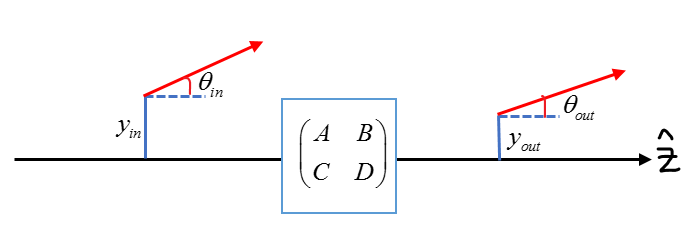
\includegraphics[width=\textwidth]{./paraxial-approx.png}
תנאי הקירוב: $\displaystyle \theta \approx \dv{y}{z} \ll 1 \Leftarrow \theta \ll 1$

$$ \mqty(y_{out} \\ \theta_{out}) = \mqty(A & B \\ C & D)\mqty(y_{in} \\ \theta_{in}) $$

\textbf{אם יש כמה מטריצות, לזכור להכפיל אותן לפי הסדר!}

% TODO: Consider adding an image of multiple matrices

\renewcommand{\arraystretch}{1.2}
% \newcommand{\centered}[1]{\begin{tabular}{l} #1 \end{tabular}}
\begin{tabular}{|>{\centering\arraybackslash} m{0.45\textwidth}|c|}
    \hline
    \adjincludegraphics[
	width=0.45\textwidth,
	trim={
	    0 {0\height} 0 0
	},
	clip
    ]{./paraxial-d-distance.png} &
    $\displaystyle \mqty(
    1 & d \\
    0 & 1) $
    \\\hline
    מראה ניצבת לציר $z$ &
    $\displaystyle \mqty(
    -1 & 0 \\
    0 & 1) $
    \\\hline
    \adjincludegraphics[
	width=0.45\textwidth,
	trim={
	    0 {0.35\height} 0 0
	},
	clip
    ]{./paraxial-convex.png}
    &
    $\displaystyle \mqty(
    1 & 0 \\
    \displaystyle \frac{n_{in} - n_{out}}{R \cdot n_{out}} & \displaystyle \frac{n_{in}}{n_{out}})$
    \\\hline
\end{tabular}
\renewcommand{\arraystretch}{1}

\nc{\foreignlanguage{hebrew}{
עדשות
}}
\vspace*{-2em}

ניקח את המטריצות לעיל עם
$n \equiv n_{lens}/n_{air}$

\vspace{0.5em}

\adjincludegraphics[
    width=\textwidth,
    trim={
	0 {0.15\height} 0 0
    },
    clip
]{./paraxial-lens.png}

$$ M =
\mqty(
\displaystyle 1- \frac{d}{R_1} (1 - n) & \displaystyle d \cdot n \\
\displaystyle -\frac{1}{f} & \displaystyle 1+\frac{d}{R_2} (1- n)
)
$$

$$
\frac{1}{f} = \left(n - 1\right)\left(\frac{1}{R_1} - \frac{1}{R_2} + \frac{d}{R_1 R_2} \left(1 - \frac{1}{n}\right)
\right)
$$

\vspace*{-0.5em}

\end{hebrew}

\end{minipage}
};
\node[fancytitle, left=10pt] at (box.north east) {\foreignlanguage{hebrew}{
אופטיקה גאומטרית בקירוב הפרקסיאלי
}};
\end{tikzpicture}

%---------------------------
\begin{tikzpicture}
\node [mybox] (box){
\begin{minipage}{0.3\textwidth}
\begin{hebrew}
\nc{\foreignlanguage{hebrew}{
עדשות
}}
\vspace*{-3em}

\begin{itemize}
\item בעדשות דקות $\abs{R_{1,2}} \gg d$.
\item לשים לב לסימן של הרדיוסים $R_{1,2}$ בהצבה ב-$\frac{1}{f}$.
\item מפזרת $f<0\iff$, מרכזת $f>0\iff$.
\end{itemize}

\nc{\foreignlanguage{hebrew}{
תנאי הדימות
}}
\vspace*{-2em}

נתונה מערכת אופטית כלשהי עם מטריצה
$M_{lens}$
ונתון גוף הממוקם במרחק
$u$
מהעדשות על הציר האופטי. תנאי הדימות הינו התנאי שהמטריצה

$$
M_{tot} =
\mqty(1 & u \\ 0 & 1) M_{lens} \mqty(1 & v \\ 0 & 1)
\overset{\bigtriangleup}{=} \mqty(A & B \\ C & D)
$$

תקיים
$\underline{B = 0}$.
תמונה וירטואלית הינה תמונה שתנאי זה גורר
$v < 0$. עבור עדשה דקה:

$$M_{lens} = \mqty(1 & 0 \\ -\frac{1}{f} & 1) \Rightarrow \frac{1}{f} = \frac{1}{u} + \frac{1}{v}$$

\nc{\foreignlanguage{hebrew}{
מישורים ראשיים
}}
\vspace*{-2em}

כמו בתנאי הדימות, עבור מערכת אופטית כלשהי עם מטריצה
$M_{lens} = \mqty(a & b \\ c & d)$,
המישורים הראשיים הם מישורים הממוקמים במרחקים
$u$
ו-
$v$
\textbf{ממרכז} המערכת האופטית
$M_{lens}$
כך ש:
\vspace*{-1.5em}

$$
M_{tot} =
\mqty(1 & u \\ 0 & 1) M_{lens} \mqty(1 & v \\ 0 & 1)
\overset{\bigtriangleup}{=} \mqty(1 & 0 \\ \displaystyle -\frac{1}{f_{eff}} & 1)
$$

פתרונות:

$$\begin{array}{lcccr}
    \displaystyle -\frac{1}{f_{eff}} = c & &
    \displaystyle u = \frac{1 - a}{c} & &
    \displaystyle v = \frac{1 - d}{c}
\end{array}$$

\end{hebrew}

\end{minipage}
};
\node[fancytitle, left=10pt] at (box.north east) {\foreignlanguage{hebrew}{
אופטיקה גאומטרית בקירוב הפרקסיאלי
}};
\end{tikzpicture}

%---------------------------
\begin{tikzpicture}
\node [mybox] (box){
\begin{minipage}{0.3\textwidth}
\begin{hebrew}

\vspace*{-0.5em}
\nc{\foreignlanguage{hebrew}{
הקירוב הפרקסיאלי:
}}
\vspace*{-2em}

מציבים במשוואת הגלים פתרון:
$\vb{E}(\vb{r}) = u(\vb{r}) e^{i (\omega t - k z)} \vu{x}$ -
גל המתקדם רק בכיוון
$\vu{z}$
ומשתמשים בקירוב:
$\displaystyle \abs{\dv[2]{u}{z}} \ll \abs{k \dv{u}{z}}$ -
מעטפת הגל משתנה במרחב לאט יותר מאורך הגל. מקבלים:

$$\laplacian_{\bot} u(\vb{r}) = \pdv[2]{u}{x} + \pdv[2]{u}{y} = 2 i k \pdv{u}{z}$$

\vspace*{-0.5em}

\end{hebrew}
\end{minipage}
};
\node[fancytitle, left=10pt] at (box.north east) {\foreignlanguage{hebrew}{
משוואת הלמהולץ
}};
\end{tikzpicture}

%---------------------------
\begin{tikzpicture}
\node [mybox] (box){
\begin{minipage}{0.3\textwidth}
\begin{hebrew}

\nc{\foreignlanguage{hebrew}{
פתרון למשוואת הלמהולץ המקורבת:
}}
\vspace*{-2em}

$$ u(x,y,z) = \frac{u_0}{z} \exp(-i k \frac{x^2 + y^2}{2 z}) $$

\nc{\foreignlanguage{hebrew}{
מעבר דרך אלמנטים אופטיים
}}
\vspace*{-2em}

\begin{multicols}{2}
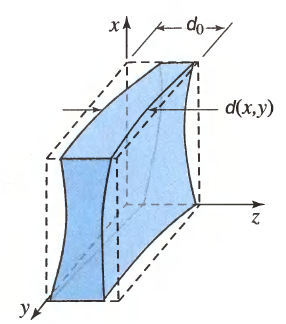
\includegraphics[width=0.5\textwidth]{./helmholtz-transition.png}
\columnbreak

$$\begin{array}{c}
\vb{E}(\vb{r}) \overset{def}{=} U(\vb{r}) e^{i \omega t} \vu{x} \\
k_0 = 2\pi/\lambda_{air} \\
\\
t(x,y) \overset{def}{=} \displaystyle \frac{U(x,y,d_0)}{U(x,y,0)} \\
\\
h_0 = e^{-i k_0 d_0}\\
\boxed{t(x,y) = h_0 e^{-i (n -1) k_0 d(x,y)}}
\end{array}$$

\end{multicols}

עדשה:

$$d(x,y) = d_0 - \frac{x^2 +y^2}{2 R} \Rightarrow t(x,y) = h_0 \exp(i k_0 \frac{x^2 + y^2}{2 f})$$

כאשר
$f = \frac{R}{n -1}$.
אפשר כך לקבל גל מישורי אם נעביר גל פרבולואידי היוצא מ-
$z = f$
ולהפך.

\end{hebrew}
\end{minipage}
};
\node[fancytitle, left=10pt] at (box.north east) {\foreignlanguage{hebrew}{
גלים פרבולואידים
}};
\end{tikzpicture}

%---------------------------
\begin{tikzpicture}
\node [mybox] (box){
\begin{minipage}{0.3\textwidth}
\begin{hebrew}

גם
$u'(x,y,z) = u(x,y,z+i z_0)$
יפתור את משוואת הלמהולץ. נגדיר:

$$\begin{array}{cc}
    \displaystyle q(z) = z + i z_0 &
    \displaystyle \frac{1}{q(z)} = \frac{1}{R(z)} - i \frac{\lambda}{\pi W^2(z)} \\
    \displaystyle W_0^2 = \frac{\lambda z_0}{\pi} = \frac{2 z_0}{k} &
    \displaystyle W^2(z) = W_0^2 \left( 1 + \left(\frac{z}{z_0}\right)^2 \right) \\
    \displaystyle \xi(z) = \arctan(\frac{z}{z_0}) &
    \displaystyle R(z) = z \left( 1 + \left(\frac{z_0}{z}\right)^2 \right)
\end{array}$$

$$\begin{array}{ll}
    U(x,y,z) = \{\rho^2 = x^2 + y^2 \} = \\
\displaystyle \boxed{\frac{A_0 W_0}{W(z)}
\exp(-\frac{\rho^2}{W^2(z)} - i\left( k z + k \frac{\rho^2}{2 R(z)} - \xi(z) \right))}
\end{array}$$

\vspace{-1em}

\end{hebrew}
\end{minipage}
};
\node[fancytitle, left=10pt] at (box.north east) {\foreignlanguage{hebrew}{
גלים גאוסיים
}};
\end{tikzpicture}

%---------------------------
\begin{tikzpicture}
\node [mybox] (box){
\begin{minipage}{0.3\textwidth}
\begin{hebrew}

\nc{\foreignlanguage{hebrew}{
    תכונות אלגבריות
}}
\vspace{-2.5em}

$$I(\rho,z) = I_0 \left ( \frac{W_0}{W(z)} \right )^2 \exp(-2\frac{\rho^2}{W^2(z)})$$

\begin{itemize}
\item $W(z)/2$ -
סטיית התקן במישור הניצב לציר
$\vu{z}$
\item $W_0 = W(z=0)$ -
רוחב
(\textenglish{Waist})
מינימלי.
\item $I(\rho=0,z) \sim \abs{U}^2 \sim \frac{1}{z_0^2 + z^2}$ -
לורנציאן.
\item $\frac{W_0}{z_0}\abs{z} \approx W(z) \Leftarrow z_0 \ll z$.
\item $\theta_0 \equiv \frac{W_0}{z_0} = \frac{\lambda}{\pi W_0}$ -
זווית ההתבדרות.
\item $R(z)$ -
רדיוס העקמומיות של הפרבולואיד.
\end{itemize}
\vspace{-2.5em}

$$
    V_{phase}(z) =
    \omega \left(\pdv{\phi(z)}{z}\right)^{-1} \approx c \left (
	1 + \frac{2 W_0^2}{k^2 W_0^4 + 4 z^2}
    \right )
$$
\vspace{-1em}

\nc{\foreignlanguage{hebrew}{
    מדידת איכות קרן
}}
\vspace*{-1.5em}

$$TODO$$

% $$M^2 \overset{def}{=} \frac{2 W_m \cdot 2 \theta_m}{4 \lambda / \pi}$$

% מודדים את
% $W$
% בכמה
% $z$ים שונים, ומבצעים התאמה

\nc{\foreignlanguage{hebrew}{
    מעבר במערכת אופטית.
}}
\vspace*{-1.5em}

\adjincludegraphics[
    width=0.9\textwidth,
    trim={
	0 {0.1\height} 0 {0.1\height}
    },
    clip
]{./abcd-gaussian.png}

מתקיים:
$\displaystyle \boxed{q_2 = \frac{A q_1 + B}{C q_1 + D}}$.
בעדשה דקה עם אורך מוקד
$f$,
עם קרן גאוסית שה-
\textenglish{Waist}
שלה ב-
$z$
נקבל:

$$\begin{array}{ccl}
    \displaystyle \frac{1}{f} = \frac{1}{R_1(z)} + \frac{1}{R_2(z)} & &
    \displaystyle W_{0,2} = M W_{0,1} \\
    \displaystyle \abs{W_1(z)} = \abs{W_2(z)} & &
    \displaystyle z_{0,2} = M^2 z_{0,1} \\
    \displaystyle M = \frac{\abs{\frac{f}{z-f}}}{\sqrt{1 + \left ( \frac{z_0}{z-f} \right )^2}} & &
    \displaystyle \theta_{0,2} = \frac{\theta_{0,1}}{M}
\end{array}$$

$$\begin{array}{c}
    \displaystyle z = f \Rightarrow M = \frac{f}{z_0} \Rightarrow W_{0,2} = \theta_{0,1} f = \frac{\lambda f}{\pi W_{0,1}}\\
    \displaystyle z = 0, z_0 \gg f \Rightarrow M \approx \frac{f}{z_0} \Rightarrow W_{0,2} \approx \theta_{0,1} = \frac{\lambda f}{\pi W_{0,1}}
\end{array}$$

\end{hebrew}
\end{minipage}
};
\node[fancytitle, left=10pt] at (box.north east) {\foreignlanguage{hebrew}{
גלים גאוסיים
}};
\end{tikzpicture}

%---------------------------
\begin{tikzpicture}
\node [mybox] (box){
\begin{minipage}{0.3\textwidth}
\begin{hebrew}
$$ f(x,y) =
\int_{-\infty}^{\infty}\int_{-\infty}^{\infty} F(\nu_x,\nu_y) e^{-2\pi i(\nu_x x + \nu_y y)} d\nu_x d\nu_y
$$
$$
F(\nu_x, \nu_y) =
\int_{-\infty}^{\infty}\int_{-\infty}^{\infty} f(x,y) e^{2\pi i(\nu_x x + \nu_y y)} dx dy
$$
\begin{center}
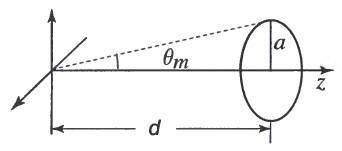
\includegraphics[width=0.85\textwidth]{./fourier-theta_m.png}
\end{center}
\vspace{-2em}
$$\begin{array}{lcl}
    \theta_x = \lambda \nu_x = 
    \sin(\theta_m)\cos(\phi) 
    & & \theta_\bot^2 = \theta_x^2 + \theta_y^2 = \sin^2(\theta_m) \\
    \theta_y = \lambda \nu_y =
    \sin(\theta_m)\sin(\phi)
    & & \nu_\bot^2 = \nu_x^2 + \nu_y^2
\end{array}$$

%\overset{\theta_\bot \ll \theta_z < 1}{\approx}\theta_m\cos(\phi)
%\overset{\theta_\bot \ll \theta_z < 1}{\approx}\theta_m\sin(\phi)

פונקצית תמסורת של מערכת אופטית הלוקחת
$f(x,y)$
והופכת אותה ל-
$g(x,y)$
מוגדרת להיות:

$$H(\nu_x, \nu_y) = \frac{F(\nu_x,\nu_y)}{G(\nu_x,\nu_y)}$$

פונקציית התגובה להלם
$h(x,y) = \mathcal{F}^{-1}[H(\nu_x,\nu_y)]$
מקיימת:

\vspace*{-1em}

$$g(x,y) = f \circledast h = \iint f(x',y') h(x-x', y-y') \dd x' \dd y'$$

בתווך חופשי -
$H_d(\nu_x, \nu_y) = \exp(-i 2 \pi \frac{d}{\lambda} \sqrt{1 - \theta_\bot^2})$

\nc{\foreignlanguage{hebrew}{
קירוב
\textenglish{Fresnel}
}}
\vspace*{-2em}

עבור רב וקטורי הגל
$\vb{k}$
מתקיים הקשר הגיאומטרי:

$$\theta_{\perp}^2 = \lambda^2 \nu_{\perp}^2 \ll 1 \Rightarrow \theta_{\perp}^2 \approx \theta_m^2 \approx \frac{a^2}{d^2} $$

הקירוב ניכר בהזנחת הסדר הרביעי ב
$ \theta_{\perp} $
של
הפאזה ב-
$H_d$:

$$ 2 \cdot \frac{d}{\lambda} \frac{\theta_m ^4}{8} = \frac{a^4}{4 \lambda d ^3} \overset{N_F \equiv \frac{a^2}{\lambda d}}{=} N_F \frac{\theta_m^2}{4} \ll 1$$

שגורר:

\vspace*{-1em}

$$\begin{array}{lcl}
    \displaystyle H_d(\nu_x, \nu_y) \approx H_{0d} \exp(-i 2 \pi \frac{d}{\lambda} \frac{\theta_m ^2}{2}) & &
    \displaystyle H_{0d} = e^{-i k d} \\
    \displaystyle h_d(x,y) \approx h_{0d} \exp(-i k \frac{x^2 + y^2}{2 d})
    & & \displaystyle h_{0d} = \frac{i}{\lambda d} e^{-i k d}
\end{array}$$

\vspace*{-1em}

$$g_d(x,y) = h_{0d} \iint f(x',y') e^{-i \frac{\pi}{\lambda d} \left (
(x - x')^2 + (y - y')^2
\right )} \dd x' \dd y'$$

\vspace*{-1em}

\end{hebrew}
\end{minipage}
};
\node[fancytitle, left=10pt] at (box.north east) {\foreignlanguage{hebrew}{
אופטיקת פורייה
}};
\end{tikzpicture}

%---------------------------
\begin{tikzpicture}
\node [mybox] (box){
\begin{minipage}{0.3\textwidth}
\begin{hebrew}

\nc{\foreignlanguage{hebrew}{
קירוב
\textenglish{Fraunhofer} -
\textenglish{"Far Field"}
}}
\vspace*{-2em}

קירוב זה בה לתת ביטוי פשוט לפונקצית התגובה להלם
$h_d(x,y)$.
ע"י פתיחת הארגומנט שלה:
$$
(x - x')^2 + (y - y')^2
 =
\underbrace{x^2+y^2}_{\le a_{out}^2} + \underbrace{x'^2+y'^2}_{\le a_{in}^2} - 2(xx'+yy')
$$
נוכל לזהות את שני זוגות האיברים הראשונים כשטחים שתופסים הגל היוצא והגל הנכנס בהתאמה. ע"י דרישת הקירוב:

$$\begin{array}{lcr}
\displaystyle N_{F,i} = \frac{a_i^2}{\lambda d} \ll 1 & & i \in \{in,out\}
\end{array}$$
כך שפונקציית התגובה להלם תקיים:

$$
g_d(x,y) \approx h_{0d} \iint f(x',y') e^{2i \frac{\pi}{\lambda d} \left (xx'+yy'\right )} \dd x'\dd y'
$$
$$\begin{array}{lcr}
  = h_{0d} F \left( \frac{x}{\lambda d},\frac{y}{\lambda d} \right) & &
\end{array}$$

\nc{\foreignlanguage{hebrew}{
עדשות -
\textenglish{"Near Field"}
}}
\vspace*{-2em}

כפי שראינו באופטיקה גיאומטרית:

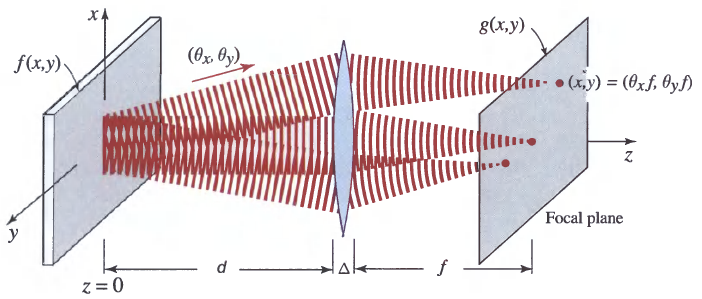
\includegraphics[width=\textwidth]{./fourier-lens.png}

עדשה מוסיפה פאזה לגלים מישוריים
$\Phi_\ell(x,y) = \pi \frac{x^2 + y^2}{\lambda f}$.
לכן תחת קירוב
\textenglish{Fresnel}
בלבד:

$$g_\ell(x,y) = \left (f(x,y) \circledast h_d(x,y) e^{i \Phi_\ell(x,y)} \right) \circledast h_f(x,y)$$
$$\begin{array}{lcr}
    = h_{0\ell} e^{i \pi (d -f) \frac{x^2+y^2}{\lambda f}} \cdot 
    F(\frac{x}{\lambda f}, \frac{y}{\lambda f}) & &
    h_{0\ell} = \frac{i}{\lambda f} e^{-i k (f +d)} 
\end{array}$$

$$I_\ell(x,y) = \abs{g_\ell(x,y)}^2 \propto \abs{F(\frac{x}{\lambda f}, \frac{y}{\lambda f})}^2$$

$$ f = d \Rightarrow g_\ell(x,y) = \frac{i}{\lambda f} e^{-i k 2 f} F(\frac{x}{\lambda f}, \frac{y}{\lambda f})$$

\end{hebrew}
\end{minipage}
};
\node[fancytitle, left=10pt] at (box.north east) {\foreignlanguage{hebrew}{
אופטיקת פורייה
}};
\end{tikzpicture}

%---------------------------
\begin{tikzpicture}
\node [mybox] (box){
\begin{minipage}{0.3\textwidth}
\begin{hebrew}

\nc{\foreignlanguage{hebrew}{
אפקט
\textenglish{Talbot}
}}
\vspace*{-2em}

יהי שריג המתפקד כמסיכה של "מסרק הלמים":
$\sum_{m=-\infty}^\infty \delta(x - m a)$
אזי במרחקים
$Z_t \cdot \alpha$
מהמסיכה כאשר:

$$\begin{array}{lcr}
\alpha \in \mathbb{Q} & &
\displaystyle Z_t = \frac{\lambda}{1- \sqrt{1 - \frac{\lambda^2}{a^2}}} \underbrace{\approx}_{\text{Fresnel} / \lambda \ll a} 2 \frac{a^2}{\lambda} 
\end{array}$$

תתקבל עוצמה כמו ב-
$z = 0$.

\nc{\foreignlanguage{hebrew}{
זהויות פוריה
}}
\vspace*{-4em}
\begin{center}
\renewcommand{\arraystretch}{1.9}
\begin{tabular}{|c|c|}
    \hline $\mathcal{F}[f] = F$ & $f$ \\\hline
    $\displaystyle e^{-2\pi i a \nu_x} F(\nu_x)$            &
    $\displaystyle f(x-a)$ \\\hline
    $\displaystyle F(\nu_x - \nu_0)$                        &
    $\displaystyle e^{-2\pi i \nu_0 x} f(x)$ \\\hline
    $\displaystyle \abs{a} F(a \nu_x)$    &
    $\displaystyle f(x/a)$ \\\hline
    $\displaystyle \abs{\lambda d} f(-\nu_x \lambda d)$     &
    $\displaystyle F(\frac{x}{\lambda d})$ \\\hline
    $\displaystyle F(\nu_x) \circledast G(\nu_x)$           &
    $\displaystyle f(x) \cdot g(x)$ \\\hline
    $\displaystyle F(\nu_x) \cdot G(\nu_x)$ &
    $\displaystyle f(x) \circledast g(x)$ \\\hline
    $\displaystyle \abs{a} \sinc(a \nu_x)$ &
    $\displaystyle \rect(\frac{x}{a}) = \begin{cases}
    1   & \displaystyle \abs{\frac{x}{a}} < \frac{1}{2} \\
    1/2 & \displaystyle \abs{\frac{x}{a}} = \frac{1}{2} \\
    0   & \displaystyle \abs{\frac{x}{a}} > \frac{1}{2}
    \end{cases}$ \\\hline
    $\displaystyle \abs{a} \rect(a \nu_x)$ &
    $\displaystyle \sinc(\frac{x}{a}) = \frac{a \sin(\pi x/a)}{\pi x}$ \\\hline
    %$\displaystyle \frac{1}{\abs{a}} \tri(\frac{\nu_x}{a}) =
    %\frac{1}{\abs{a}} \begin{cases}
    %\displaystyle 1- \abs{\frac{\nu_x}{a}} & \displaystyle \abs{\frac{\nu_x}{a}}<1 \\
    %0 & \text{Otherwise}
    %\end{cases}$ &
    %$\displaystyle \sinc^2(a x)$ \\\hline
    %$\displaystyle \frac{1}{\abs{a}} \sinc^2(\frac{\nu_x}{a})$ &
    %$\displaystyle \tri(a x)$ \\\hline
    %$\displaystyle \sqrt{\frac{\pi}{\alpha}} e^{-\frac{(\pi \nu_x)^2}{\alpha}}$ & 
    %$\displaystyle e^{-\alpha x^2} $ \\\hline
    %$\displaystyle \frac{\2 a}{a^2 + 4 \pi^2 \nu_x^2}$ & 
    %$\displaystyle e^{-a \abs{x}} $ \\\hline
    $\begin{array}{c}
        \displaystyle \frac{J_1(2\pi R \nu_\bot)}{R \nu_\bot} \\
        \begin{cases}
        \displaystyle \rho = \sqrt{x^2 + y^2} \\
        \displaystyle \nu_\bot = \sqrt{\nu_x^2 + \nu_y^2} \\
        \end{cases}
    \end{array}$ &
    $\displaystyle circ(\rho/R) = \begin{cases}
    1 & \rho < R \\
    1/2 & \rho = R \\
    0 & \rho > 0
    \end{cases}$ \\\hline
    %$\frac{1}{\nu_\bot}$ &
    %$\frac{1}{\rho}$ \\\hline
    $\displaystyle \delta(\nu_x - \nu_0)$ &
    $\displaystyle e^{2\pi i \nu_0 x}$ \\\hline
    $\displaystyle \frac{1}{a} \sum_{m=-\infty}^{\infty} \delta(\nu_x - \frac{m}{a})$ &
    $\displaystyle \sum_{m=-\infty}^{\infty} \delta(x - m a)$ \\\hline
    $\displaystyle \frac{\abs{a}}{2}\left ( \frac{1}{i \pi a \nu_x} + \delta(a \nu_x) \right)$ &
    $\displaystyle \Theta(\frac{x}{a}) = \begin{cases}
    1   & \frac{x}{a} > 0 \\
    1/2 & x = 0 \\
    0   & \frac{x}{a} < 0
    \end{cases}$ \\\hline
\end{tabular}
\renewcommand{\arraystretch}{1}
\end{center}
\vspace{-1em}

\end{hebrew}
\end{minipage}
};
\node[fancytitle, left=10pt] at (box.north east) {\foreignlanguage{hebrew}{
אופטיקת פורייה
}};
\end{tikzpicture}

%---------------------------
\begin{tikzpicture}
\node [mybox] (box){
\begin{minipage}{0.3\textwidth}
\begin{hebrew}

\begin{multicols}{2}
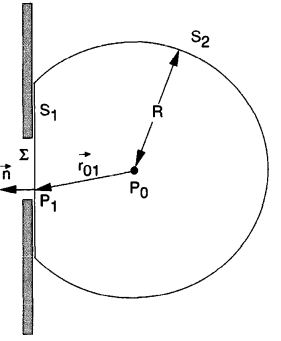
\includegraphics[width=0.5\textwidth]{./diffraction.png}
\columnbreak

נתון מפתח כדורי עם שפה
$S_1$
המכסה את כל השטח באיזור הנקודה
$\vb{P_0}$
חוץ מבמפתח
$\Sigma$.
נרצה לחשב את אמפליטודת השדה החשמלי
$U(\vb{P_0})$.

משתמשים במשפט גרין עבור
$U$
ו-
$G$
ובעובדה שהן מקיימות את משוואת הלמהולץ. קירכהוף בחר:

\vspace*{-1.5em}
$$G_{\vb{P_0}}(\vb{r}) =
\frac{e^{-i k \abs{\vb{r} - \vb{P}_0}}}
{\abs{\vb{r} - \vb{P_0}}}
$$

\end{multicols}
%הנושא מכליל את כל מה שעשינו באופטיקת פורייה ונותן לנו נקודת מבט שונה. 
%בתחום של המרחב בו אנו מסתכלים תחת פונקצית גרין כגל כדורי:

$$ U(\vb{P_0}) =\frac{1}{4\pi} \oiint_S \dd s \left( \pdv{U}{n}G_{\vb{P_0}} -U\pdv{G_{\vb{P_0}}}{n} \right) $$
עבור 
$R\to \infty $
האינטגרל על 
$S_2$
מתאפס אם מתקיים תנאי
\textbf{\textenglish{Sommerfeld radiation condition}}:

$$\lim _{R\to \infty} R\left[ ikU - \pdv{U}{n} \right] =0$$

ומקבלים:

$$ U(\vb{P_0}) =\frac{1}{4\pi} \iint_{\Sigma} \dd s \left( \pdv{U}{n}G_{\vb{P_0}} -U\pdv{G_{\vb{P_0}}}{n} \right) $$

$$\pdv{G_{\vb{P_0}}}{n} = \left (-i k - \frac{1}{\abs{\vb{r} -
\vb{P}_0)}}\right ) G_{\vb{P_0}} \cdot \cos(\angle(\vu{n},\vb{r} -\vb{P_0}))$$

\nc{\foreignlanguage{hebrew}{
הפתרון של 
\textenglish{Sommerfeld}
}}
\vspace*{-2em}

נגדיר
$\vb{P'_0}$
שיקוף של
$\vb{P_0}$
ונקרב:
$ \abs{\vb{r} - \vb{P_0}}^{-1} \ll k $
ונקבל:

$$
G_\pm (\vb{r})= G_{\vb{P_0}}(\vb{r}) \pm G_{\vb{P'_0}}(\vb{r}) \Rightarrow
\eval{G_{-}(\vb{r})}_\Sigma = \eval{\pdv{G_{+}(\vb{r})}{n}}_\Sigma=0
$$

$$\pdv{G_{-}(\vb{r})}{n} = -2\cos(\angle(\vu{n},\vb{r} -\vb{P_0}))\cdot i k G_{\vb{P_0}}(\vb{r}) $$

$$U(\vb{P_0}) =\frac{1}{i\lambda} \iint_{\Sigma} \cos(\angle(\vu{n},\vb{r} -\vb{P_0})) U(\vb{r}) G_{\vb{P_0}}(\vb{r}) \dd s$$

$$U(\vb{P_0}) = \frac{1}{4 \pi} \iint_{\Sigma} \pdv{U}{n} G_{+}({\vb{r}}) \dd s = \frac{1}{2 \pi} \iint_{\Sigma} \pdv{U}{n} G_{\vb{P_0}}({\vb{r}}) \dd s$$
\vspace{-1em}

\end{hebrew}
\end{minipage}
};
\node[fancytitle, left=10pt] at (box.north east) {Diffraction - \foreignlanguage{hebrew}{
עקיפה
}};
\end{tikzpicture}

%---------------------------
\begin{tikzpicture}
\node [mybox] (box){
\begin{minipage}{0.3\textwidth}
\begin{hebrew}

\nc{\foreignlanguage{hebrew}{
קריטיריון
\textenglish{Rayleigh}
}}

\vspace{-2em}

עונה על השאלה:
\textit{
מה המרחק המינימלי בין שני חרירים כדוריים שנוכל להבדיל ביניהם ב-
\textenglish{"Far Field"}?
}
מניחים שלשני החרירים קוטר
$D$
והם מרוחקים זה מזה מרחק
$\rho_s > D/2$
כלומר:

\vspace{-1em}

$$f(x,y) = circ(\frac{\sqrt{x^2 + y^2}}{D/2}) + circ(\frac{\sqrt{(x-\rho_s)^2 + y^2}}{D/2})$$

הפונקציה

\vspace{-1em}

$$\mathcal{F}[circ(\frac{\rho}{D/2})] = \frac{J_1(2\pi \frac{D}{2} \nu_\bot)}{\frac{D}{2} \nu_\bot} \overset{def}{=} \frac{D^2\pi}{2} \Jinc(\pi D \nu_\bot)$$

מתאפסת ב-
\textenglish{"Far Field"}
עבור
$\nu_\bot = \frac{x_0}{\lambda d}$
ב-
$x_0 \approx 1.22 \frac{\lambda d}{D}$.
לכן נדרוש שהמרחק בין החרירים יקיים:

$$\rho_s > x_0 \approx 1.22 \frac{\lambda d}{D}
\underbrace{\gg}_\text{Fraunhofer} D$$

\nc{\foreignlanguage{hebrew}{
בעדשה - גל גאוסייני
}}
\vspace{-2em}

נתונה עדשה עם קוטר
$D$
ומוקד
$f$
ממוקמת ב-
$z=0$
של גל גאוסי עם
$z_{0,1} \gg f$.
העוצמה של הגאוסיין מתפרסת על כל המישור
$z=0$
לכן נבחר שרירותית קוטר סופי
$D = 2 W_{0,1}$
ונקבל:

$$\begin{array}{lcr}
    \displaystyle W_{0,2} \approx \frac{2\lambda}{\pi}\cdot \frac{f}{D} = \frac{2\lambda}{\pi}\cdot F_{\#} & &
    \displaystyle F_{\#} \overset{def}{=} \frac{f}{D} \\
\end{array}$$

\nc{\foreignlanguage{hebrew}{
בעדשה - גלים פרבולואידיים
}}
\vspace{-2em}

\begin{multicols}{2}
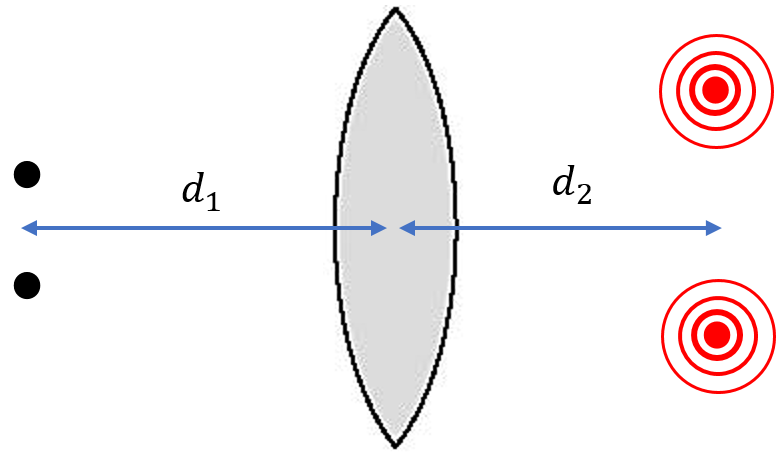
\includegraphics[width=0.5\textwidth]{resolution-lens-point-source.png}
\columnbreak

בדומה לקריטריון
\textenglish{Rayleigh}
ניקח מקורות נקודתיים של גלים פרבולואידיים ונשאל 
\textit{
מה המרחק המינימלי ביניהן שנוכל להבדיל ביניהן ב-
$d_2$?}
נניח תנאי דימות
$\frac{1}{d_1} + \frac{1}{d_2} = \frac{1}{f}$
וקוטר
$D$
לעדשה.

\end{multicols}

נחשב את האמפליטודה במוצא של מקור נקודתי פרבולואידי על ציר
$\vu{z}$.
נשתמש גם בטריק מתמטי לפיו:

\vspace{-2em}

$$\text{\{עדשה בקוטר
\{D} = \text{\{חריר בקוטר
\{D}\dotproduct \{\infty\text{\{עדשה בקוטר
}$$

\vspace{-0.5em}

מקבלים:

\vspace{-1em}

$$g_{out}(x,y) \sim \Jinc(\frac{x}{\lambda d_2}, \frac{y}{\lambda d_2}) \Rightarrow \rho_s > x_0 \approx 1.22 \frac{\lambda d_2}{D}$$

\vspace{-1em}

\end{hebrew}
\end{minipage}
};
\node[fancytitle, left=10pt] at (box.north east) {\foreignlanguage{hebrew}{
רזולוציה אופטית
}};
\end{tikzpicture}

%---------------------------
\begin{tikzpicture}
\node [mybox] (box){
\begin{minipage}{0.3\textwidth}
\begin{hebrew}

שיטה לשמירת אינפורמציה תלת מימדית על נייר פילם. אינפורמציה תלת-מימדית טמונה בפאזה היחסית בין נקודות שונות באובייקט הממוקמות רחוק/קרוב יותר לנייר הצילום. תיאור השיטה:

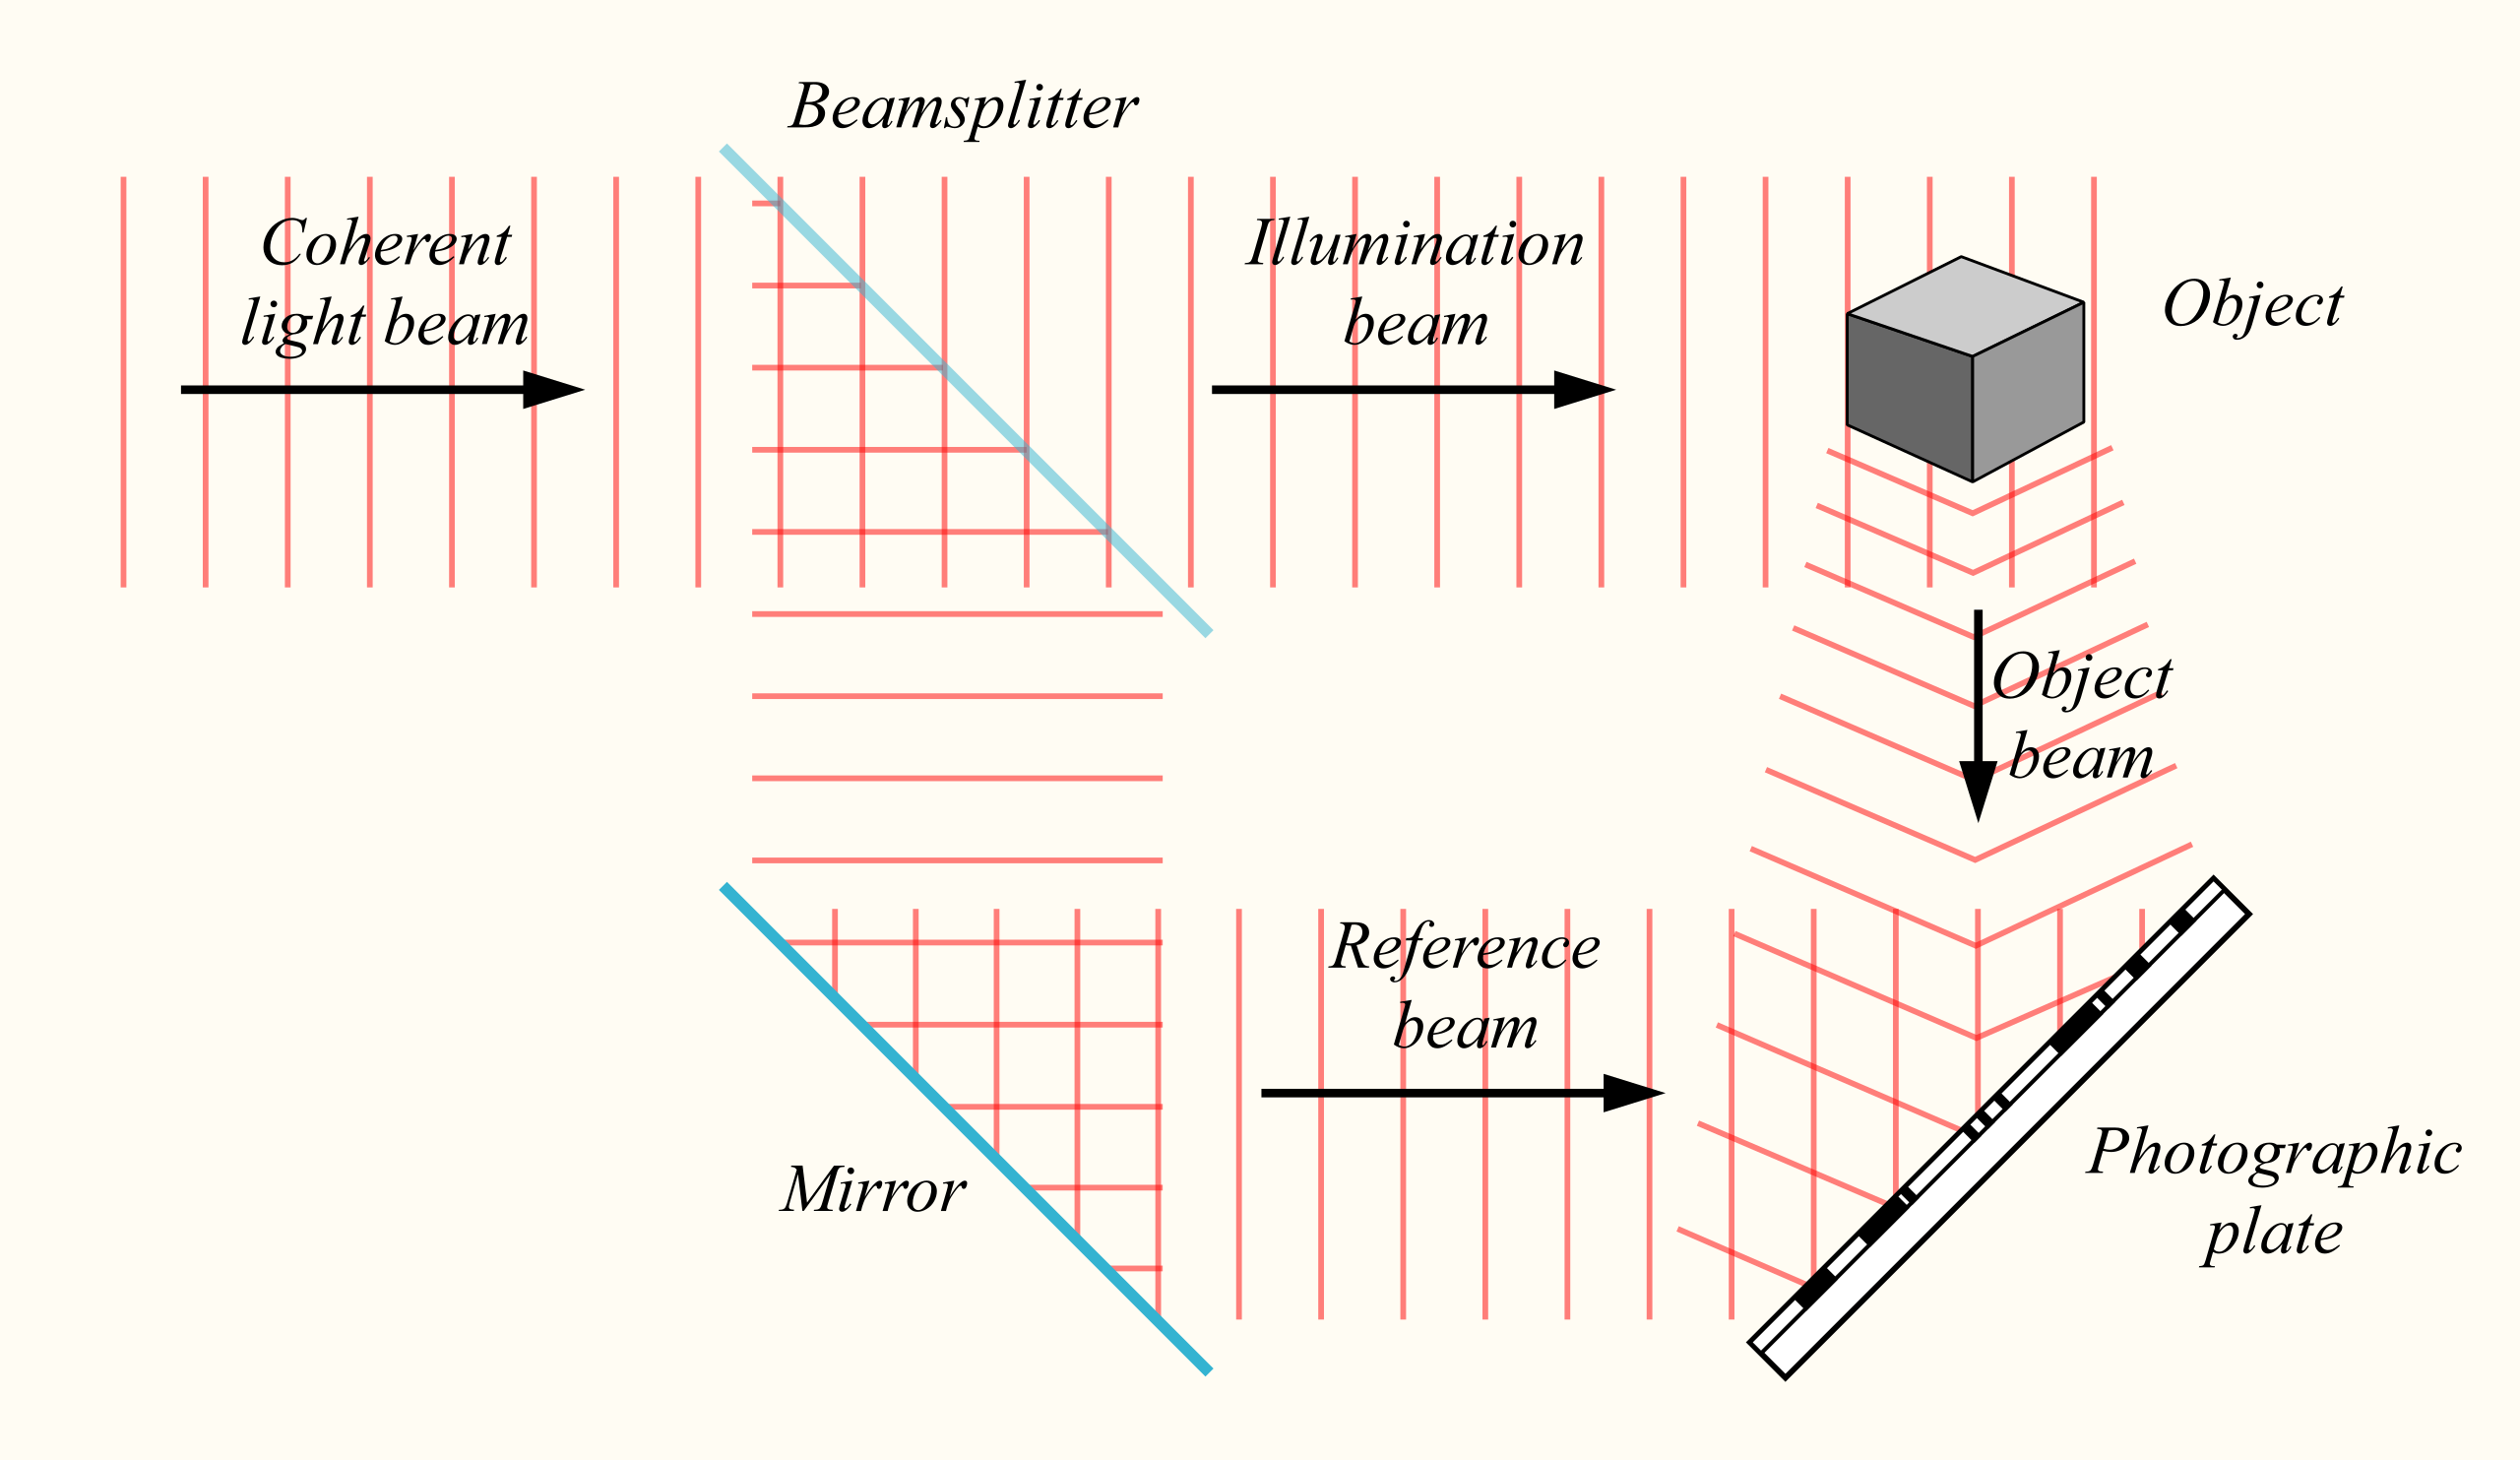
\includegraphics[width=\textwidth]{Holography-record.png}

נייר הפילם רגיש לעוצמה של האור הפוגע בו. נסמן את האור הקוהרנטי ב-
$U_r$,
את השדה היוצא מהאובייקט ב-
$U_o$
ואת התמונה הנשמרת בפילם ב-
$t$:

$$t = \abs{U_o + U_r}^2 = I_o + I_r + \underbrace{2\real\mathrm{e} \{U_r^*U_o\}}_{\text{לא קיים בצילום רגיל}}$$

לאחר מכן משחזרים את התמונה באמצעות גל
$U_r$
כמו בעת הצילום ומקבלים על המסך:

\vspace{-0.5em}

%$$U = U_r \cdot t = I_o U_r + I_r U_r + 2 U_r \real\mathrm{e} \{U_r^*U_o\}$$
$$U_{out} = 
U_r \cdot t = 
\underbrace{I_o U_r + I_r U_r}_\text{רקע לא מעניין} + 
\underbrace{I_r U_o}_{\text{שחזור}} +
\underbrace{U_r^2 U_o^*}_{\text{דמות צמודה}}$$

\begin{multicols}{2}
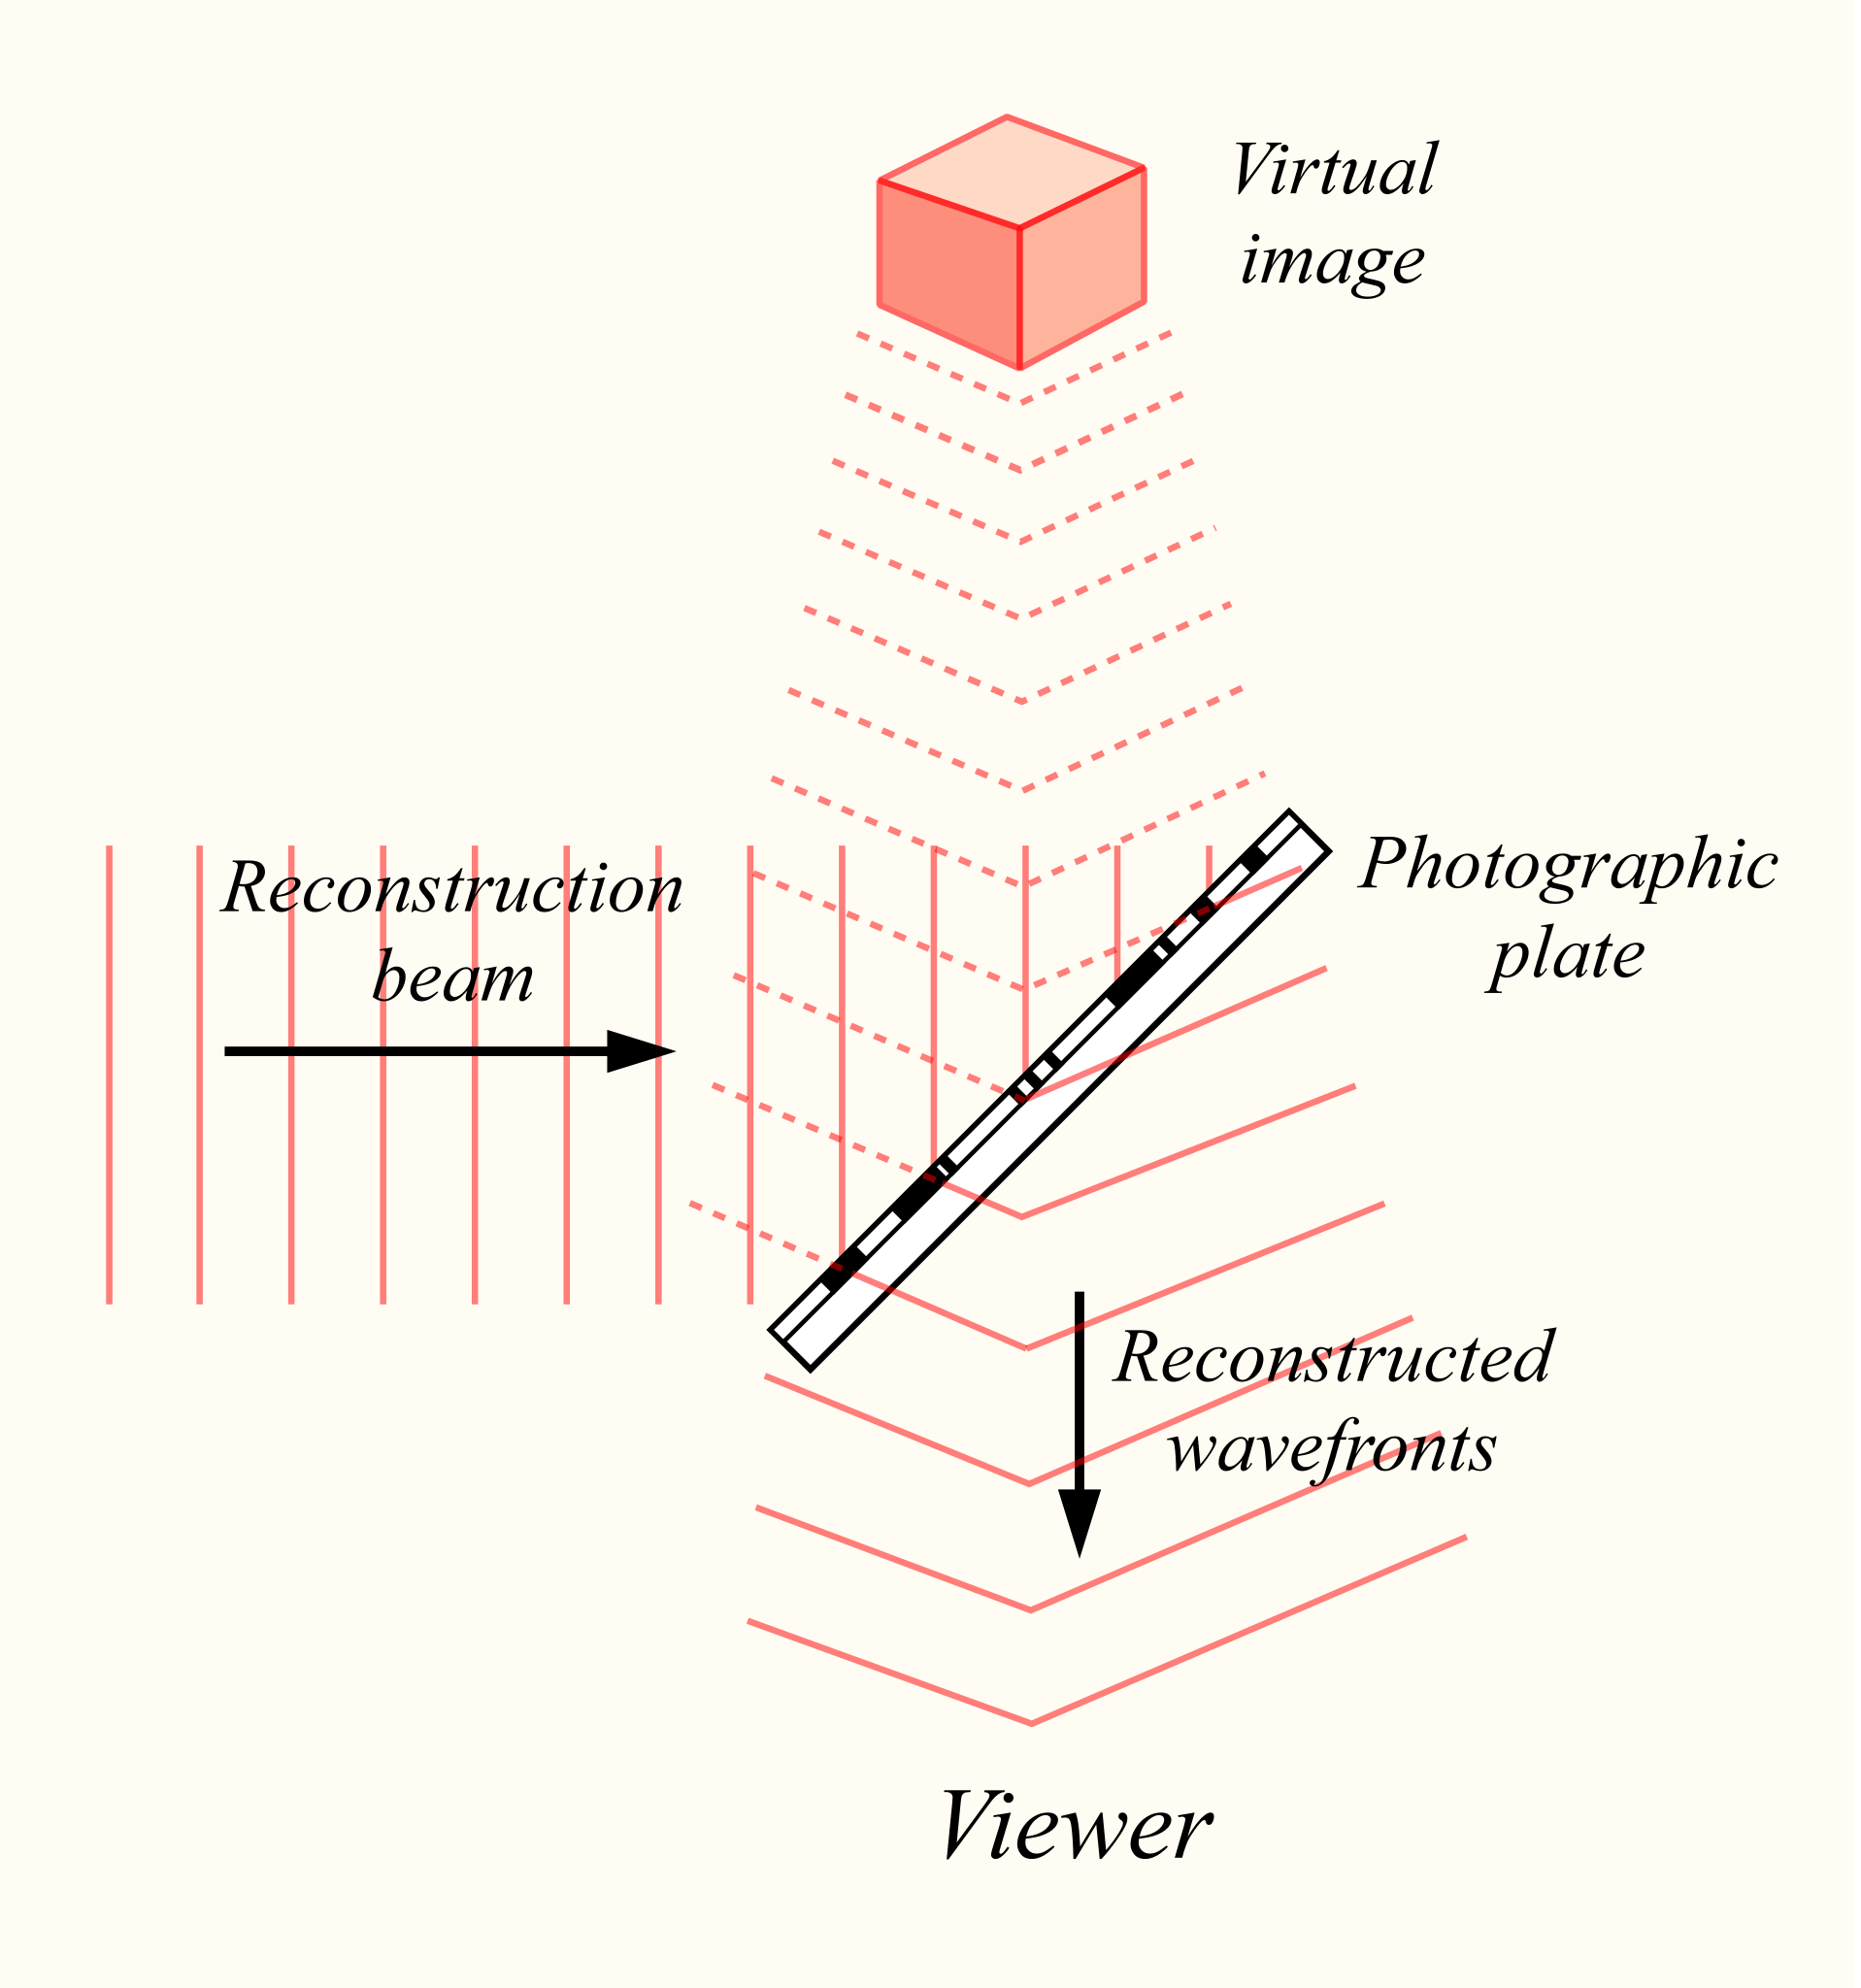
\includegraphics[width=0.5\textwidth]{Holography-reconstruct.png}
\columnbreak

\begin{itemize}[itemsep=3pt]
\item המרחק שעובר הגל
$U_r$
דרך האובייקט ודרך המראה צריך להיות דומה, עד כדי אורך הקוהרנטיות של המקור.
\item המערכת צריכה להיות יציבה בסקלות של אורך הגל ב-
$U_r$.
\end{itemize}

\end{multicols}
\vspace{-1.5em}

\end{hebrew}
\end{minipage}
};
\node[fancytitle, left=10pt] at (box.north east) {\foreignlanguage{hebrew}{
הולוגרפיה
}};
\end{tikzpicture}

\begin{adjustbox}{center}\begin{tikzpicture}
\cat[body=gray,nose=red]
\end{tikzpicture}\end{adjustbox}

%---------------------------
\begin{tikzpicture}
\node [mybox] (box){
\begin{minipage}{0.3\textwidth}
\begin{hebrew}

פונקצית האוטוקורלציה:
\small$$
G(\tau)  = \left< U^*(t) U(t+\tau)  \right> = \lim _{T\to \infty} \frac{1}{T} \int ^{\frac{T}{2}}_{-\frac{T}{2}}  U^*(t) U(t+\tau) \dd t
$$\normalsize

"המנורמלת":
$$\begin{array}{lcr}
\displaystyle g(\tau)=\frac{G(\tau)}{G(\tau = 0)} & & \displaystyle 0\le g(\tau) \le 1
\end{array}$$

זמן קוהרנטיות
$ \tau_c$
ואורך קוהרנטיות 
$ l_c$
מקושרים ע"י מהירות האור
$c$:
$$ \tau_c = \frac{l_c}{c} = \int_{-\infty}^{\infty} \abs{g(\tau)}^2\dd \tau $$

מתוך התמרת פורייה של העוצמה:

$$ U_T(f)=\int_{-\frac{T}{2}}^{\frac{T}{2}} U(t)\cdot e^{-2\pi i f t} \dd t$$

נקבל את ההגדרה ל -
\textenglish{Power Spectral Density}
:

$$ S(f)=\lim_{T \to \infty} \frac{1}{T} \abs{U_T(f)}^2 = \mathcal{F} \left[ G(\tau) \right] (f) $$

כך שהעוצמה של הגל מקיימת:

$$ I=G(\tau=0)=\int_0^\infty S(f) \dd f $$

נוכל להבחין שוב מתוך משפטי פרסבל והתמרות פורייה כי ההגדרות עד כה מקיימות:

$$ \tau_c = \frac{\int_0^\infty \abs{S(f)}^2 \dd f}{\left( \int_0^\infty S(f) \dd f \right)^2} \equiv \frac{1}{\Delta \nu_c}$$

כאשר
$\Delta \nu_c$
הרוחב הספקטרלי של הגל.

\nc{\foreignlanguage{hebrew}{
קוהרנטיות מרחבית
}}
\vspace*{-2em}

אוטוקורלציה מרחבית:

$$ G(\vb{r}_1, \vb{r}_2,\tau) = \expval{U^*(\vb{r}_1,t) U(\vb{r}_2,t+\tau)} $$

"המנורמלת" המרחבית:

$$ \begin{array}{lcr}
    \displaystyle g(\vb{r}_1, \vb{r}_2,\tau) = \frac{G(\vb{r}_1, \vb{r}_2,\tau)}{\sqrt{I(\vb{r}_1) I(\vb{r}_2)}} & &
    \displaystyle I(\vb{r}) = \expval{U^*(\vb{r},t) U(\vb{r},t)}
\end{array}$$

באופן דומה לזמן הקוהרנטיות, ניתן להגדיר רוחב ספרטקלי חדש,
$l^*_c$,
המתאר את המרחק בין הנקודות בו המנורמלת המרחבית 
$g(\vb{r}_1, \vb{r}_2,0)$
דואכת לגובה מוסכם.

\end{hebrew}
\end{minipage}
};
\node[fancytitle, left=10pt] at (box.north east) {\foreignlanguage{hebrew}{
קוהרנטיות
}};
\end{tikzpicture}

%---------------------------
\begin{tikzpicture}
\node [mybox] (box){
\begin{minipage}{0.3\textwidth}
\begin{hebrew}

\nc{\foreignlanguage{hebrew}{
התאבכות של מקורות שונים
}}
\vspace*{-2em}

פונקציית הקרוסקורלציה "המנורמלת" בין שני מקורות עם אמפליטודות
$U_1,U_2$
היא:

$$g_{12}(\vb{r}_1, \vb{r}_2,\tau) =
    \frac{\expval{U_1^*(\vb{r}_1, t) U_2(\vb{r}_2, t+\tau)}}
         {\sqrt{I_1(\vb{r}_1) I_2(\vb{r}_2)}}
$$

היתרון בהגדרה זו היא בעוצמת ההתאבכות בין שני המקורות:

%$$ I_{tot}(\vb{r}_1, \vb{r}_2) = I_1(\vb{r}_1) +I_2(\vb{r}_2) + 2\sqrt{I_1I_2}\real\mathrm{e}\{{g_{12}(\vb{r}_1, \vb{r}_2, \tau = 0)}\}$$

$$ I_{tot}= I_1+I_2 + 2\sqrt{I_1 I_2} \cdot \real\mathrm{e}\{{g_{12}(\tau = 0)}\}$$


כך שנוכל להגדיר את ה -
\textenglish{Visibility}
להיות:
$$ V = \frac{2 \sqrt{I_1I_2}}{I_1+I_2}\real\mathrm{e}\{{g_{12}}\}$$

יחס זה נותן לנו את נראות ההתאבכות בין שני המקורות.

\end{hebrew}
\end{minipage}
};
\node[fancytitle, left=10pt] at (box.north east) {\foreignlanguage{hebrew}{
קוהרנטיות
}};

\end{tikzpicture}

\end{multicols*}
\end{document}